\chapter{Deployment of the application(CI/CD)}\label{sect:cicd}

\subsection*{Overview}
\tab CI/CD \cite{cicd} (continuous integration/continuous delivery) is a way for delivering apps to clients on a regular basis by incorporating automation into the app development process. Continuous integration, continuous delivery, and continuous deployment are the three key principles associated with CI/CD. CI/CD is a solution to the challenges that development and operations teams face while integrating new code (AKA "integration hell").

\tab CI/CD, in particular, adds continuous automation and monitoring across the app lifecycle, from integration and testing through delivery and deployment. These approaches are referred to as a "CI/CD pipeline" when they are combined, and they are supported by development and operations teams working together in an agile manner using either a DevOps or a site reliability engineering (SRE) strategy.

\subsection*{What is the distinction between CI and CD (and other CDs)?}
\tab There are a number possible meanings for the abbreviation CI/CD. The "CI" in CI/CD stands for continuous integration, which is a developer automation method. New code changes to an app are built, tested, and merged to a common repository on a regular basis with successful CI. It's a solution to the problem of having too many app branches in development at the same time that could conflict.

\tab Continuous delivery and/or continuous deployment are related ideas that are sometimes used interchangeably in the CI/CD acronym. Both are about automating pipeline stages farther down the line, although they're sometimes used independently to show how much automation is taking place.

\tab Continuous delivery often means that a developer's modifications to an application are immediately bug checked and published to a repository (such as GitHub or a container registry), from which the operations team may deploy them to a live production environment. It's a solution to the issue of lack of visibility and communication between development and business teams. To that end, the goal of continuous delivery is to make it as easy as possible to deploy new code.

\tab Continuous deployment (another alternative "CD") refers to a developer's changes being automatically released from the repository to production, where they can be used by customers. It tackles the issue of operations staff being overburdened with manual processes that hinder app delivery. It extends the benefits of continuous delivery by automating the pipeline's next stage.

\begin{center}
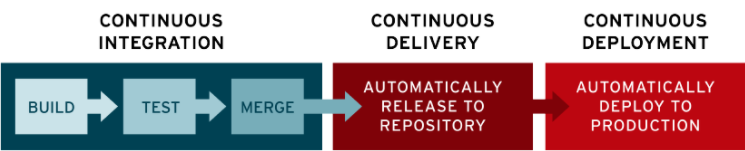
\includegraphics[width=400pt]{cicd image.PNG} 
\end{center}

\tab CI/CD can refer to merely the related practises of continuous integration and continuous delivery, or it can refer to all three connected practises of continuous integration, delivery, and deployment. To make matters more confusing, the term "continuous delivery" is sometimes used to refer to both continuous delivery and continuous deployment methods.

\tab In the end, it's probably not worth your time to get mired down in these semantics—just remember that CI/CD is a process that involves adding a high degree of ongoing automation and continuous monitoring to app development, and it's commonly depicted as a pipeline.

\tab What the phrases refer to varies depending on how much automation has been incorporated into the CI/CD pipeline on a case-by-case basis. Many businesses begin by using CI and then progress to automated delivery and deployment in the future, such as as part of cloud-native apps.

\tab Our expertise can assist your company in establishing the techniques, tools, and culture required to more effectively modernise existing applications and develop new ones.

\subsection*{Continuous integration}
\tab The goal of modern application development is to have numerous developers working on different aspects of the same programme at the same time. However, if a company is set up to combine all branching source code on a single day (known as "merge day"), the work that results can be tedious, manual, and time-consuming. That's because when a developer working alone makes a change to an application, there's a potential it'll clash with other modifications being made at the same time by other developers. If each developer has created their own local integrated development environment (IDE), rather than the team agreeing on a single cloud-based IDE, the problem can be exacerbated.

\tab Continuous integration (CI) enables developers to merge changes to a shared branch, or "trunk," more frequently—even daily. Once a developer's modifications to an application have been merged, the changes are validated by generating the app automatically and running various levels of automated testing, often unit and integration tests, to confirm the changes haven't broken the programme. This entails testing everything from classes and functions to the various modules that make up the programme as a whole. If automated testing uncovers a conflict between new and existing code, continuous integration (CI) makes it easier to fix errors fast and frequently.

\subsection*{Continuous delivery}
\tab Continuous delivery automates the deployment of validated code to a repository after the builds and unit and integration testing are automated in CI. As a result, it's critical that CI be already built into your development pipeline if you want to have a successful continuous delivery process. The purpose of continuous delivery is to have a codebase that is always ready to go into production.

\tab Every level of continuous delivery incorporates test automation and code release automation, from merging code changes through delivering production-ready builds. At the end of the procedure, the operations team is able to swiftly and efficiently deploy an app to production.

\subsection*{Continuous deployment}
\tab Continuous deployment is the final stage of a mature CI/CD workflow. Continuous deployment is an extension of continuous delivery, which automates the release of a production-ready build to a code repository. It also automates the release of an app to production. Continuous deployment relies significantly on well-designed test automation because there is no manual gate at the point of the pipeline before production.

\tab Continuous deployment, in practise, means that a developer's change to a cloud application could go live minutes after being written (assuming it passes automated testing). This makes it much easy to acquire and implement user feedback on a regular basis. All of these connected CI/CD methods, when combined, make application deployment less dangerous, as it's easier to deliver changes to apps in little chunks rather than all at once. However, because automated tests would need to be built to handle a range of testing and release phases in the CI/CD pipeline, there will be a significant upfront investment.

\subsection*{What are some common CI/CD tools?}
\section {Maven}

\tab Maven \cite{introducing_maven}, a Yiddish phrase that means "collector of knowledge," originated as an attempt to streamline the Jakarta Turbine project's construction processes. There were multiple projects, each with its own Ant build files, that were slightly different from one another. CVS was used to check in JARs. We needed a common way to build projects, a clear definition of what a project was, a simple way to publish project information, and a means to exchange JARs across several projects.

\tab As a result, you now have a tool that can be used to create and manage any Java-based project. We hope that we have built something that will aid in the understanding of any Java-based project and make the day-to-day job of Java developers easier.

\subsection*{Maven's Objectives}
\tab Maven's main purpose is to help developers understand the entire status of a development project in the quickest amount of time possible. Maven tackles a number of issues in order to achieve this goal:

\begin{itemize}
    \item Streamlining the delivery process
    \item Providing a standardised build system
    \item Delivering high-quality project data
    \item Better development approaches are encouraged.
\end{itemize}

\subsection*{Making the build process simple}
\tab While Maven does not remove the need to understand the underlying mechanics, it does shelter developers from many of the complexities.

\subsection*{Providing a standardized build system}
\tab Maven uses its project object model (POM) and a set of plugins to create a project. Once you've learned how to build one Maven project, you'll be able to build any Maven project. When navigating many projects, this saves time.

\subsection*{Providing high-quality project data}
\tab Maven provides useful project information that is derived in part from your POM and in part from the sources of your project. Maven, for example, can provide:

\begin{itemize}
    \item Directly from source control, a change log is generated.
    \item Sources with cross-references.
    \item The project's mailing lists are administered by the project.
    \item Dependencies utilised by the project.
    \item Unit test reports including coverage.
\end{itemize}

\tab Third-party code analysis packages also provide Maven plugins that supplement Maven's basic information with their own findings.

\subsection*{Providing guidelines for best practices development}
\tab Maven's goal is to compile current best practises development concepts and make it simple to steer a project in that direction.

\tab The formulation, execution, and reporting of unit tests, for example, are all part of the standard Maven build cycle. As a guide, the following current unit testing best practises were used:

\begin{itemize}
    \item Maintaining a distinct yet parallel source tree for test code.
    \item Locating and running tests using test case naming conventions.
    \item Instead of configuring the build for test preparation, test cases should set up their environment.
    \item Maven can also help with project process issues like release and issue management.
\end{itemize}

\tab Maven also provides some instructions for laying up the directory structure of your project. Once you've mastered the layout, you'll be able to traverse other Maven-based projects with ease.

\tab While it takes an opinionated approach to project layout, historical considerations may prevent some projects from fitting into this framework. While Maven is designed to be adaptable to the needs of various projects, it cannot accommodate every circumstance without jeopardizing its goals.

\tab If your project's build structure is unique and cannot be restructured, you may have to forego some functionality or abandon Maven entirely.

\subsection*{What is Maven Not?}
\tab Some of the following things about Maven might be familiar for you:

\begin{itemize}
    \item Maven is a site-building and documentation platform.
    \item Maven is an Ant extension that allows you to download dependencies.
    \item Maven is a collection of reusable Ant scriptlets.
\end{itemize}

\tab While Maven does these things, as you can see in the "What is Maven?" section above, these aren't the only characteristics it has, and its goals are rather different.

\section {Jenkins}
\tab Jenkins® \cite{jenkins_esentials} is an open source automation server. By automating the software development process, enterprises can save time and money. Jenkins is a tool that manages and controls software delivery processes across the whole lifecycle, including build, document, test, package, stage, deployment, static code analysis, and more.

\tab Jenkins may be configured to monitor any code changes in GitHub, Bitbucket, or GitLab and do an automatic build using Maven and Gradle. You can use container technology like Docker and Kubernetes to run tests and then take actions in production like rolling back or forward.

\subsection*{Jenkins History}
\tab While working for Sun Microsystems, Kohsuke Kawaguchi founded the Jenkins project (formerly called Hudson) in 2004. Kohsuke was a Sun engineer who was fed up with his team's fury every time his code broke the build. Jenkins was designed as a technique to perform continuous integration – that is, to test his code before committing it to the repository to ensure everything was working properly. Jenkins was quickly adopted by his colleagues as they witnessed what he was accomplishing. Kohsuke made it open source, resulting in the Jenkins project, which quickly grew in popularity around the world.

\subsection*{Jenkins Today}
\tab Jenkins, which was originally created by Kohsuke for continuous integration (CI), now orchestrates the complete software delivery process, which is referred to as continuous delivery. For certain businesses, automation goes even farther, allowing for continuous deployment. Software delivery is considerably accelerated when continuous delivery (CD) is combined with a DevOps culture.

\tab Jenkins is the most extensively used continuous delivery solution, owing to its versatility and active community. Jenkins can be integrated with nearly any tool, including all of the best-of-breed solutions used throughout the continuous delivery process, thanks to the Jenkins community's more than 1,700 plugins. Jenkins continues to gain traction as the leading solution for software process automation, continuous integration, and continuous delivery, with more than 165,000 active installations and 1.65 million users worldwide as of February 2018.

\subsection*{CloudBees and the Jenkins Community}
\tab CloudBees is an active member of the Jenkins community and contributes significantly to the project's success. CloudBees employs a number of important contributors to the Jenkins project. CloudBees is the lead sponsor of DevOps World | Jenkins World, the annual user conference for the Jenkins community, in support of the community. Jenkins World brings people together, provides a sense of belonging, helps users to learn from one another, and promotes community growth. CloudBees has also aided the growth of Jenkins Area Meetups (JAMs) around the world, donating the JAMS to the CDF so that they can continue to thrive.

\tab CloudBees support and product engineers contribute code to the Jenkins project on a regular basis, participate in Jenkins chats and project meetings, and contribute to the Jenkins project email lists. Jenkins X, Jenkins Pipeline, and Jenkins 2 are just a few of the significant projects CloudBees has worked on. Furthermore, all updates made by CloudBees in the open source code are submitted back to the project, allowing us all to benefit from an ever-better Jenkins experience.

\tab Continuous Information is a monthly newsletter published by CloudBees for the Jenkins community. It's chock-full of community tips & tricks, articles, presentations, global events, and a slew of other resources. Subscribe to receive it in your inbox once a month.

\subsection*{Jenkins and the Continuous Delivery Foundation}
\tab The Linux Foundation established the Continuous Delivery Foundation (CDF) in 2019. In partnership with the Jenkins and Jenkins X communities, Google, the Linux Foundation, and others, CloudBees led the launch initiative.

\tab The CDF is dedicated to fostering, growing, and supporting open source projects, best practices, and industry standards relating to continuous delivery. Jenkins, Jenkins X, Spinnaker, and Tekton are just a few of the open source projects hosted by the CDF. More projects are likely to join, with the goal of forming a continuous delivery (CD) ecosystem to develop specifications and initiatives around portability and interoperability. CloudBees is a founding member of the initiative, and it continues to contribute technology and resources to it.

\section {Git}
\subsection*{Branching and Merging}
\tab The branching model of Git \cite{git} is what really sets it different from practically every other SCM out there.

\tab Git supports and encourages the creation of several local branches that are completely independent of one another. It takes seconds to create, merge, and delete those development lines.

\tab As a result, you can do things like:

\begin{itemize}
    \item Context Switching with No Friction. To test an idea, create a branch, commit a few times, switch back to where you branched from, apply a patch, switch back to where you're exploring, and merge it in.
    \item Codelines based on roles. Create a branch that only contains what goes to production, a branch that you merge work into for testing, and a few smaller branches for day-to-day work.
    \item Workflow that is based on features. Create different branches for each new feature you're working on so you can transition between them effortlessly, then delete each branch after the feature is integrated into your main line.
    \item Experimentation with Disposables. Create a branch to experiment in, discover it's not going to work, and simply remove it, abandoning the task (even if you've pushed other branches in the meantime).
\end{itemize}

\begin{center}
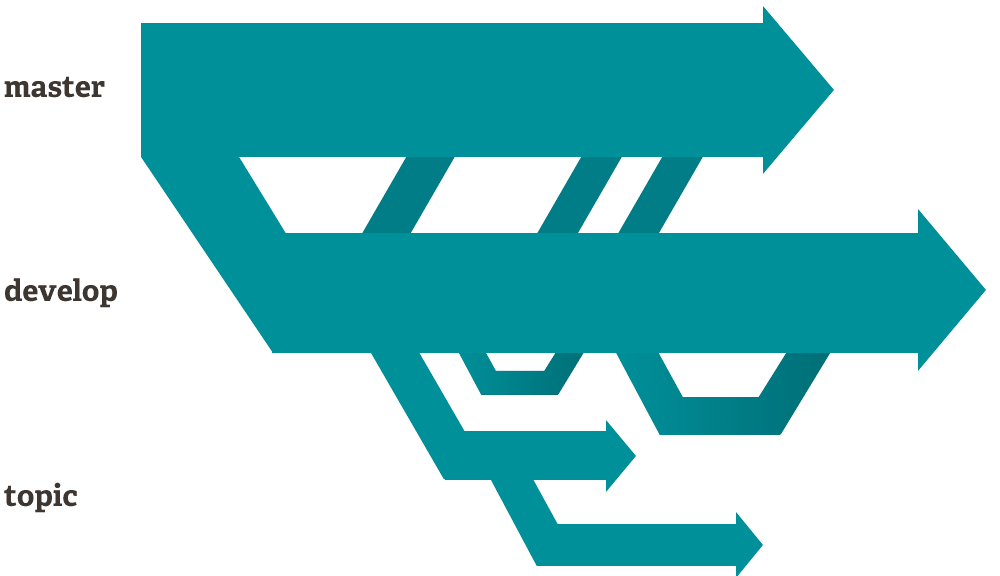
\includegraphics[width=400pt]{git.png} 
\end{center}

\tab You don't have to push all of your branches to a remote repository, for example. You have the option of sharing just one, a couple, or all of your branches. This allows people to experiment with new ideas without having to worry about how and when they will integrate them or share them with others.

\tab Some of this can be accomplished using other methods, but the job is far more complicated and error-prone. Git makes this process incredibly simple, and once learned, it transforms the way most engineers operate.